\documentclass[11pt,a4paper,twoside,twocolumn]{article}

%--------------- Packages -------------------------------------------------
\usepackage{graphicx,parskip,times,amsfonts,amsmath}
\usepackage{jacobs-research-report}
\usepackage{eurosym}
\usepackage{natbib}
\usepackage{a4,a4wide}
\usepackage[latin1]{inputenc}
\usepackage[english]{babel}
\usepackage{amssymb,amsmath,amsfonts}
\usepackage{bibunits}
\usepackage{longtable}
\usepackage{bpchem}
%---------------------PDF-definitions--------------------------------------
\usepackage[pdftex,           %%% hyper-references for pdflatex
  hypertexnames=false,%       %%% needed for correct links to figures
  breaklinks=true,%           %%% break links if exceeding a single line
  colorlinks=true,%           %%% to underline links instead of boxing
  urlcolor=blue]{hyperref}    %%% blue instead of cyan URLS
%--------------------end-of-PDF-definitions-------------------------------
\usepackage{makeidx}
\makeindex

%--------------------User Definitions----------------------------------------
\hyphenation{Schlei-cher} \hyphenation{geo-me-try}
\newcommand{\C}{\mathbb{C}}
\newcommand{\R}{\mathbb{R}}
\usepackage{latexsym}
\newcommand{\bbbr}{\mathbb{R}}
\newcommand{\bbbn}{\mathbb {N}}
\newcommand{\bbbc}{\mathbb {C}}
\newcommand{\mycaption}[1]{\caption{#1}}
\renewcommand*{\cleardoublepage}{\clearpage\if@twoside \ifodd\c@page\else
    \hbox{}
    \if!\blankpagetext!\else
    \vfil \begin{center} \setlength{\fboxsep}{3mm}%
    \framebox{\blankpagetext}
    \end{center}\vfil\vfil \fi
    \newpage\if@twocolumn\hbox{}\newpage\fi\fi\fi}
\newcommand*{\resetpages}{\cleardoublepage\pagenumbering{arabic}}
\raggedbottom \pagenumbering{Roman}
\newenvironment{myitemize}{\begin{list}{-}{\labelwidth=0.2cm \leftmargin0.4cm
\labelsep0.2cm \rightmargin0cm \parsep0.5ex plus0.2ex minus0.1ex
\itemsep0ex
 plus0.2ex}}{\end{list}}

% new line after paragraph heading
\makeatletter
\newcommand\myparagraph{%
\@startsection{paragraph}{4}{\z@}%
{-3.25ex \@plus1ex \@minus.2ex}%
{.15ex \@plus.1ex \@minus.1ex}%
{\normalfont\normalsize\bfseries}}
\makeatother

\setlength{\parskip}{0pt plus 1pt}

%---------------------- Document ------------------------------------------------
\begin{document}
\def\Hchapter{\paragraph}
\def\bpchem{\BPChem}
%---------------- Path for images and pictures -------------------------------------
\graphicspath{{./MathTheoPhys/}{./Nano/}{./LifeSciences/}{./ESS/}{./EECS/}}
%----------------Title -------------------------------------------------------------
\title     {School of Humanities and Social Sciences\\
            Research Report 2007/2008} \shorttitle{RP 2007/2008}
\author    {Freia Hardt}
\date      {2009 January}
\masterfile{SHSS--RR--2007/2008}
\issue     {0}
\revision {1}
\version {2}{0}{05.01.09}{Test}
%-----------------------------------------------------------------------------------
\renewcommand{\refname}{\medbreak Publications\vadjust{\nobreak}}
\renewcommand{\bibname}{\medbreak Publications\vadjust{\nobreak}}
%-----------Table of Contents one column -------------------------------------------
\onecolumn
\shorttitle{Table of Contents} \tableofcontents \resetpages

%----------- Switch to two columns ----------------------------------------------------
\twocolumn

%------------ Into Dean ---------------------------------------------------------------
%\input{xxx}
\cleardoublepage
% Each chapter starts on a right page
\ 

%
%
\subsubsection{Cellular and Wireless Communications}
\label{Haas1} \index{Haas, Harald}

\paragraph{Research Team}
Harald Haas (Professor), Rami Abu-Alhiga (PhD Student), Zubin
Bharucha (PhD Student), Hany Elgala (PhD Student), Ellina Foutekova
(PhD Student), Birendra Ghimire (PhD Student), Dennis Kolyuzhnov
(PhD Student),  Raed Youself Mesleh (PhD Student), Abdurazak Mudesir
(PhD Student), Hrishikesh Venkataraman (PhD Student), Sinan
Sinanovic (Research Associate), Peter Omiyi (Postdoc), Mostafa
Afgani (Research Engineer), Sudharasan Ganesan (Graduate Student)\\

Research in Cellular and Wireless Communications is geared towards
new technologies. Particular focus is  on the development and the
interaction of key air-interface building blocks \newpage

\begin{myitemize}
\item multicarrier transmission (in particular OFDM (Orthogonal Frequency Division
Multiplexing)
\item duplexing techniques (in particular time division duplexing
(TDD))
\item multiple-input multiple-output (MIMO) techniques
\item wireless ad hoc systems
\item medium access control (MAC) algorithms
\item multiple access and scheduling techniques
\item dynamic channel assignment (DCA) algorithms
\item mobile positioning
\item visible light communication.
\end{myitemize}

\myparagraph{Highlights} \emph{Spatial Modulation.} Spatial
modulation (SM) is a new and patented multiple antenna transmission
approach for wireless systems that increases the spectral efficiency
(number of bits transmitted per Hz bandwidth) by utilizing the
transmit antenna number as an implicit source of information. A
block of information bits is mapped to an information symbol and a
transmit antenna number. As a consequence, at any given time instant
only a single antenna of the antenna array is transmitting signal
power. The actual block of information bits determines which antenna
is active at a particular time instant. As a result, inter-channel
interference (ICI) at the receiver input and the need to synchronize
the transmit antennas are completely avoided. Simple receiver
algorithms such as maximum receive ratio combining (MRRC) can be
used to retrieve the information bits. The performance and the
receiver complexity of SM and V-BLAST (Vertical-Bell Labs Layered
Space-Time) algorithm in flat fading channels are compared. V-BLAST
applies zero forcing detection based optimum ordering, nulling and
successive interference cancellation. The basic principle of SM is
depicted in Fig.~\ref{smexmpl}, and results of the comparison with
state-of-the-art V-BLAST are shown in Fig.~\ref{fig55}.
\begin{figure}[!htb]\centering
  \centerline{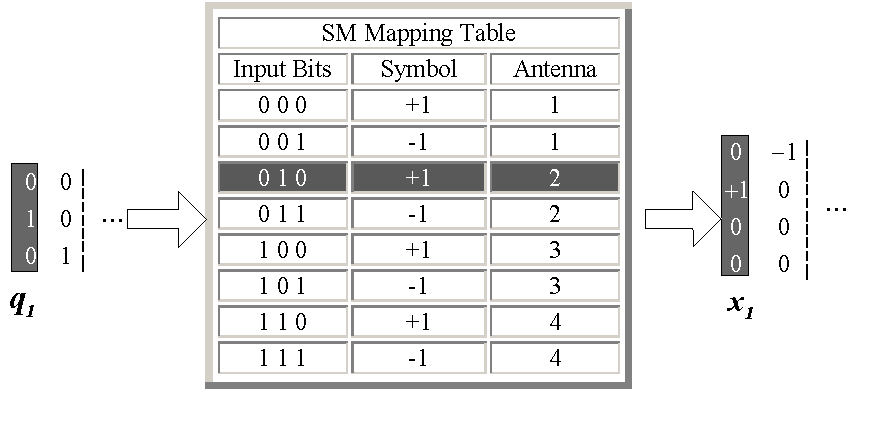
\includegraphics[width=8cm]{haas_1.pdf}}
  \caption{3bits/symbol spatial modulation mapping table using binary phase shift keying (BPSK)
    and four transmit antennas} \label{smexmpl}
\end{figure}
\begin{figure}[!!htp]\centering
  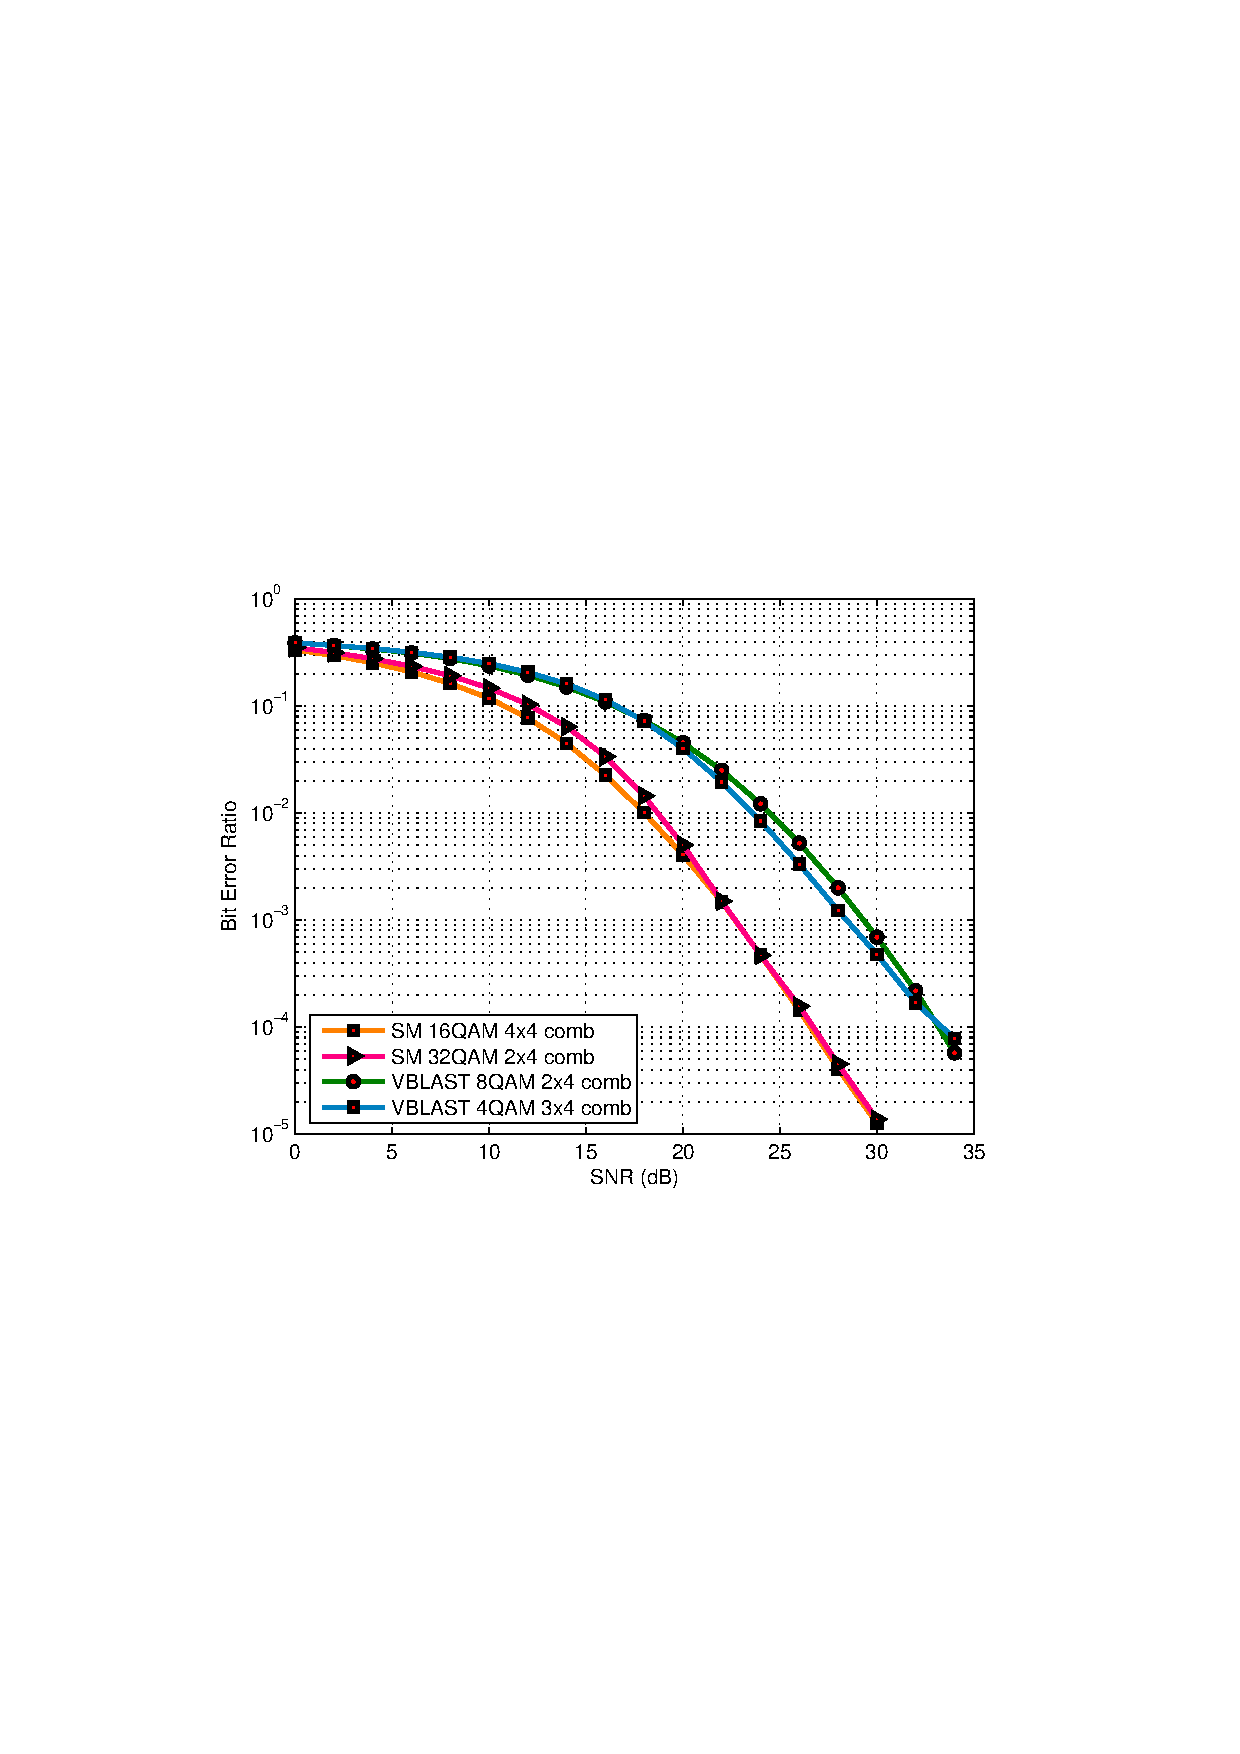
\includegraphics[width=8cm]{haas_2.pdf}\\
  \caption{Bit error performance as a function of signal-to-noise ratio (SNR) for state-of-the-art V-BLAST and novel SM.}
  \label{fig55}
\end{figure}
From the results it can be found that the performance gains are
significant. In both schemes the same number of bit per unit
bandwidth are transmitted (for fair comparison), but with SM the bit
error performance is reduced considerably. For example, at an SNR of
20dB a 10-fold reduction in the BER is observed.

\emph{Dynamic Resource Allocation.} In this work a fully
decentralized interference avoidance algorithm to manage
interference in an \emph{ad hoc} wireless network, applicable to
wireless sensor networks, is developed and analyzed. Fig.~\ref{dca}
depicts a randomly chosen distribution of transmitting (Tx) and
receiving (Rx) nodes. The new algorithm, called \emph{busy tone
interference tolerance signaling}, is of low complexity and is very
easy to implement. It is based on different functions to set the
busy tone signal power dependent on the level of tolerable
interference, and their performance is compared with a special case
of a fixed power system which provides maximum capacity assuming
equal transmit powers. Results show that an appropriately chosen
function for setting the busy-tone can lead to gains in capacity
using very little power. This power efficiency advantage is quite
significant, implying that battery life of units can be extended
while providing a similar capacity than a fixed power system.
\begin{figure}[!!htp]
 \centering
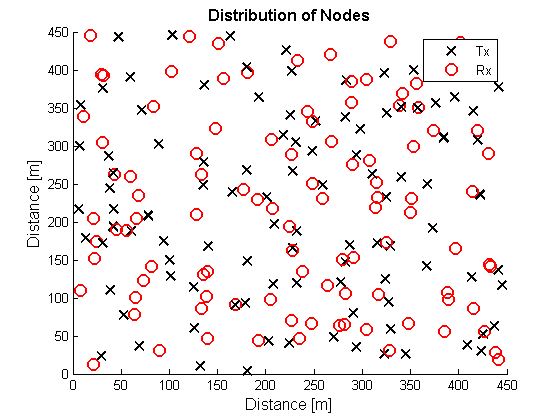
\includegraphics[width=8cm]{haas_3.png}\\
\caption{Random distribution of nodes in an \emph{ad hoc} wireless network}
\label{dca}
\end{figure}

%\null Harald Haas is also involved in ``Signal Processing''
%(Section~\ref{Haas1}).

%\newpage
\paragraph{Organization}
% list the (research) events you have organized, if any,
\begin{enumerate}
    \item Member of Technical Program Committee of and session chair
          at \emph{IEEE International Conference on Personal, Indoor \& Mobile Radio Communications} -- PIMRC 2006
    \item Member of Technical Program Committee of \emph{International IEEE Conference on Vehicular Technology} -- VTC 2006
\end{enumerate}

\paragraph{Collaborations}
\begin{enumerate}
\item {\sl The University of Edinburgh, UK}\\
  Prof. S. McLaughlin\\
  Joint project with industrial partner on \emph{Hybrid Cellular and Multihop Wireless
    Networks}
\end{enumerate}

\newpage
\paragraph{Grants}
% list the running grants in 2005, if none have been received, please delete this
% subsection.
\begin{enumerate}
    \item Funded by industry partner,
      \emph{Cellular TDD-OFDM (Time division duplex - orthogonal frequency
          division multiplexing)},  June 2004 - July 2005


    \item Funding by industry partner and University of Edinburgh, \emph{Hybrid Cellular and Multihop Wireless
    Networks},  July 2005 - July 2006

    \item Funded by industry partner, \emph{Link Adaptation and Scheduling in Cellular
    Systems},  March 2005 - February 2008

    \item Funded by Bremen T.I.M.E program funded by BIS
    Bremerhaven, \emph{Mobile Positioning (MPos)} in collaboration with MobilTec GmbH and supported by
     T-Mobile,  June 2006 - September 2009

    \item Funded by DFG Schwerpunktprogram TakeOFDM, \emph{DCA Algorithms and MAC Protocols for COFDM Based Cellular and
     Ad hoc Systems Using Carrier Sensing Time Division Multiple Access
     (CSTDMA)},  October 2004 - September 2006

\end{enumerate}

\paragraph{Patents}
% list the grants you have received in 2005, if none have been received, please delete this
% subsection.
\begin{enumerate}
\item Four new patent applications submitted
\item Three previously submitted patents got granted in 2006
\end{enumerate}

\paragraph{Awards, Prizes}
\begin{enumerate}
\item Nominated for the Chinese 111 Program -- Guest Academic Talents Programme for the Development of University Disciplines in China
\item Invited Talk at the University of Mondragon (Spain)
%    \item Honorary Fellowship of Edinburgh University
%    \item Invited to Institute for Digital Communications (IDCOM) at the University of
%          Edinburgh on \emph{Vodafone Fellowship on Communications}
    %\item Invited speaker at \emph{International Next Generation Wireless Network Workshop},
     %     Edinburgh/Scotland
\end{enumerate}

%\paragraph{Publications}
% list the publications of 2005 (also accepted and in press), if none have been received, please delete this
% subsection. Enter the publications into the SES publications database at
% http://kwarc.eecs.iu-bremen.de/ses-pubs/index.php and only reference them here.

 
\nocite{ah06_vis_light}
\nocite{bh06_ped_dead_reck}
\nocite{hnona06_iamac}
\nocite{vh06_thru_cap}
\nocite{cvh06_freq_syn}
\nocite{feh06_semi_analytic}
\nocite{fagvh06_sch_CDMA}
\nocite{jhm06_adhoc_tdd_underlay}
\nocite{oha06_tsalloc_insotdd}
\nocite{mhay06_spatialmod}
\nocite{asilomar06}
\nocite{chinacom06}
\nocite{tdd_book}
\nocite{oha07}
 

 
%\begin{bibunit}[hplain]
\begin{thebibliography}{10}

\bibitem{ah06_vis_light}
M.~Afgani and H.~Haas.
\newblock Visible light communication using {OFDM}.
\newblock In {\em Proceedings of the 2nd International Conference on Testbeds
  and Research Infrastructures for the Development of Networks and Communities
  (Trident 2006)}, Barcelona, Spain, March 01-06 2006.

\bibitem{bh06_ped_dead_reck}
S.~Beauregard and H.~Haas.
\newblock "{Pedestrian Dead Reckoning (PDR) and GPS for Indoor Positioning}".
\newblock In {\em Proceedings of 3rd Workshop on Positioning, Navigation and
  Communication ({WPNC}'06)}, Hannover, Germany, March 16 2006.

\bibitem{cvh06_freq_syn}
S.~Chaudhury, H.~Venkataraman, and H.~Haas.
\newblock "{Uplink Capacity Comparison of Non-Perfect Frequency Synchronised
  Cellular OFDM Systems}".
\newblock In {\em Proceedings of International Wireless Communications and
  Mobile Computing Conference ({IWCMC} 2006)}, Vancouver (Canada), July 3-6
  2006.

\bibitem{fagvh06_sch_CDMA}
E.~Foutekova, P.~Agyapong, B.~Ghimire, H.~Venkataraman, and H.~Haas.
\newblock "{Scheduling in Cellular TDD-CDMA Networks}".
\newblock In {\em Proceedings of the International Vehicular Technology
  Conference ({VTC}) 2006-Fall}, Montreal, Canada, September 25-28 2006. IEEE.

\bibitem{feh06_semi_analytic}
E.~Foutekova, C.~Evers, and H.~Haas.
\newblock "{Semi-Analytical Derivation of Interference in TDD-CDMA Systems
  Employing Random Time Slot Hopping (RTSH)}".
\newblock In {\em Proceedings of the International Vehicular Technology
  Conference ({VTC}) 2006-Fall}, Montreal, Canada, September 25-28 2006. IEEE.

\bibitem{asilomar06}
S.~Ganesan and H.~Haas.
\newblock "{On the Performance of Spatial Modulation OFDM}".
\newblock In {\em "{Asilomar Conference on Signals, Systems, and Computers}"},
  Monterey, CA, USA, October 30 -- November 1 2006. IEEE.

\bibitem{hnona06_iamac}
H.~Haas, V.~D. Nguyen, P.~Omiyi, N.~H. Nedev, and G.~Auer.
\newblock "{Interference Aware Medium Access in Cellular OFDMA/TDD Network}".
\newblock In {\em Proceedings of International Conference on Communications
  ({ICC} 2006)}, Istanbul, Turkey, June 11-15 2006. IEEE.

\bibitem{tdd_book}
H.~Harald and S.~McLaughlin, editors.
\newblock {\em "{Next Generation Mobile Access Technologies: Implementing
  TDD}"}.
\newblock Cambridge University Press, Spring 2007.

\bibitem{jhm06_adhoc_tdd_underlay}
P.~Jain, H.~Haas, and S.~McLaughlin.
\newblock "{Capacity Enhancement using Ad Hoc Pico-Cells and TDD Underlay}".
\newblock In {\em Proceedings of the 17th International Symposium on Personal,
  Indoor and Mobile Radio Communications ({PIMRC} 2006)}, page~5, Helsinki,
  Finland, September 11-14 2006. IEEE.

\bibitem{mhay06_spatialmod}
R.~Mesleh, H.~Haas, C.~C. Ahn, and S.~Yun.
\newblock "{Spatial Modulation -- OFDM}".
\newblock In {\em Proceedings of the International {OFDM} Workshop}, Hamburg,
  Germany, August 30-31 2006.

\bibitem{chinacom06}
R.~Mesleh, H.~Haas, C.~Wook Ahn, and S.~Yun.
\newblock "{Spatial Modulation -- A New Low Complexity Spectral Efficiency
  Enhancing Technique}".
\newblock In {\em "{ChinaCOM 2006}"}, Beijing, China, October 25 -- 27 2006.
  IEEE.

\bibitem{oha06_tsalloc_insotdd}
P.~Omiyi, H.~Haas, and G.~Auer.
\newblock "{Analysis of Intercellular Timeslot Allocation in Self-Organising
  TDD Cellular Mobile Systems}".
\newblock In {\em Proceedings of the 17th International Symposium on Personal,
  Indoor and Mobile Radio Communications ({PIMRC} 2006)}, page 5 pages on CD
  ROM, Helsinki, Finland, September 11-14 2006. IEEE.

\bibitem{vh06_thru_cap}
H.~Venkataraman and H.~Haas.
\newblock "{Throughput Capacity for 2-Hop Hybrid Cellular Networks}".
\newblock In {\em Proceedings of 6th Scandinavian Workshop on Wireless Ad-hoc
  Networks ({ADHOC} '06)}, Stockholm (Sweden), May 3-4 2006.

\end{thebibliography}
\end{bibunit}
%\subsubsection{Digital Transmission Methods and Coding}
\label{ict:cns:henkel} \index{Henkel, Werner}

\paragraph{Research Team}
Werner Henkel (Professor), Fangning Hu (PhD Student), Neele von Deetzen (PhD
Student), Khaled Shawky Hassan (PhD Student), Apirath Limmanee (PhD Student)\\

We currently concentrate on iterative decoding and unequal error protection in
coding and physical transport. In iterative decoding, we study the convergence
behavior and properties of analog Turbo-like codes and the possible design of
Turbo and LDPC codes for unequal error protection (UEP). In the design of UEP
codes, we especially cooperate with ENSEA, France, and Lule\aa\ University,
Sweden. UEP is also the goal in our multicarrier research, where we design
bit-allocation algorithms that allow for easy realization of different
protection classes in an arbitrary way. UEP will be a must for current and
especially future triple-play data services to different devices at varying
channel qualities.

The analog codes have a strong relation to signal processing. Regarding
practical applications of such codes, we especially look into the correction
of impulse-noise and clipping effects. There, the most important task is to
determine statistical properties that allow for easy erasure marking, which
would support further decoding steps, analog and digital.

We further started a project on data transmission using ultrasound signals. We
currently design lab experiments to deliver data for later modeling of the
channel and disturbances.

%%% give a very short (150 words description of your research area)
%% Hint: this can be copied from the research areas document (../masterplan/research-areas)

\paragraph{Highlights}

The design of UEP Turbo codes by a pruning approach led us to a structure that
we named hybrid concatenation, a combination of outer parallel and inner
serial concatenation. The study of the decoding convergence with so-called EXIT
charts yielded the result that the area between the curves describing the
outer iterations depend on the number of inner iterations. This allows for
minimizing the decoding complexity by a scheduling with varying number of
iterations in the different decoding steps (see Fig.~\ref{fig:henkel_1}). The
pruning concept was also the starting point for our design of UEP LDPC codes
with an irregular check-node profile (pat. pending).

\begin{figure}[ht]
  \centering
  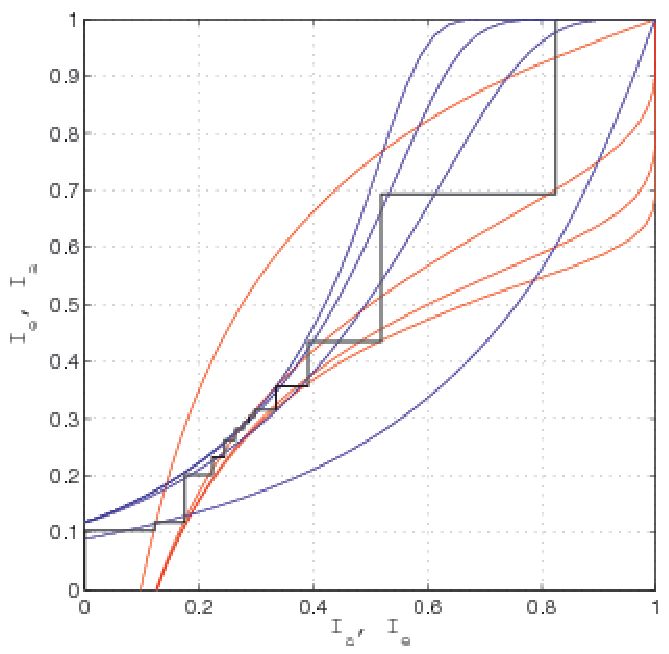
\includegraphics[width=7cm]{henkel_1}
 \caption{Convergence scheduling for hybrid concatenation}
%  \caption{Convergence scheduling for hybrid concatenation}
  \label{fig:henkel_1}
\end{figure}

In analog coding, we further improved the presentation of our proof that
Turbo-like decoding leads to a least-squares solution. We can now exactly
forecast the convergence limits for the stepsize and can also
modify it for every iteration to allow for very fast
convergence. For impulse-noise detection, we currently investigate new
statistical properties, e.g., the slope distribution, and correlation
approaches. This study will also close a gap in impulse-noise modeling
regarding the autocorrelation function of impulse noise.

By designing a new bit-allocation algorithm (pat. pending), following the
principles of an existing one by Chow, Cioffi, and Bingham, we can obtain UEP
properties in a very elegant way. It allows for an arbitrary number of
error-protection classes with arbitrary margins between them and an arbitrary
number of bits per class. Figure~\ref{fig:henkel_2} shows a resulting bit and
power allocation according to the channel SNRs, assuming three error protection
classes with a 3 dB separation.


\begin{figure}[ht]
  \centering
  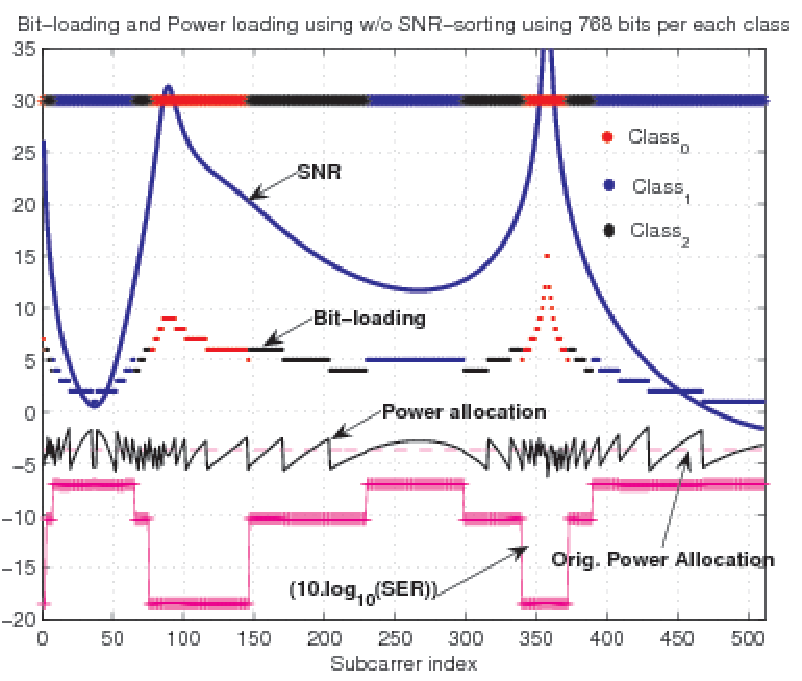
\includegraphics[width=7cm]{henkel_2}
  \caption{UEP bit and power allocation for three protection classes}
%  \caption{UEP bit and power allocation for three protection classes}
  \label{fig:henkel_2}
\end{figure}

\newpage
\paragraph{Organization}
% list the (research) events you have organized, if any,

\begin{enumerate}
\item Program Committee member of ICC 2006
\end{enumerate}

%\paragraph{Collaborations}
%\begin{enumerate}
%\item ...
%\item ...
%\item ...
%\end{enumerate}

\paragraph{Grants}
% list the running grants in 2005, if none have been received, please delete this
% subsection.
\begin{enumerate}
\item Funded by EU-IST STREP (FP 6), \emph{M-Pipe}, (October 2004
- March 2007)
\end{enumerate}

\paragraph{Patents}
\begin{enumerate}
\item  L. Sassatelli, W. Henkel, and D. Declercq. Check-Irregular LDPC Codes, Jan. 27
  2006. European Patent Application 06 100 979.1.
\item W. Henkel and K. Hassan. Unequal Error Protection Bit Loading for Multi-Carrier
  Transmission, Aug 30 2006. European Patent Application 06 119 771.1.
\end{enumerate}


%\paragraph{Publications}
% list the publications of 2005 (also accepted and in press), if none have been received, plese delete this
% subsection. Enter the publications into the SES publications database at
% http://kwarc.eecs.iu-bremen.de/ses-pubs/index.php and only reference them here.

%\begin{description}

%\item[Conference Proceedings]
  \nocite{Henkel_vDeetzen_IZS}
  \nocite{Hu_Henkel_Turbo}
  \nocite{Sassatelli_Henkel_Declercq_Turbo}
  \nocite{vDeetzen_Henkel_ISIT}
  \nocite{Henkel_Hassan_OFDM}
  \nocite{vDeetzen_ITG}
  \nocite{Hassan_Henkel_ITG}
%\item[Patents]
%  \nocite{Sassatelli_Henkel_Declercq_EP}
%  \nocite{Henkel_Hassan_EP}
%\end{description}

%%% Local Variables:
%%% mode: latex
%%% TeX-master: "report"
%%% End:

% \begin{bibunit}[hplain]\begin{thebibliography}{1}

\bibitem{Hassan_Henkel_ITG}
K.~Hassan and W.~Henkel.
\newblock {Unequal Error Protection Bit Loading in MIMO OFDM}.
\newblock In {\em ITG-Fachgruppe, 8. Sitzung}, Bremen, Oct. 6 2006.

\bibitem{Henkel_Hassan_OFDM}
W.~Henkel and K.~Hassan.
\newblock {OFDM (DMT) Bit and Power Loading for Unequal Error Protection}.
\newblock In {\em OFDM Workshop}, Hamburg, Aug 30-31 2006.

\bibitem{Henkel_vDeetzen_IZS}
W.~Henkel and N.~von Deetzen.
\newblock {Path Pruning for Unequal Error Protection Turbo Codes}.
\newblock In {\em 2006 International Z\"urich Seminar on Communications},
  Z\"urich, Switzerland, Feb. 22-24 2006.

\bibitem{Hu_Henkel_Turbo}
F.~Hu and W.~Henkel.
\newblock {A Geometric Description of the Iterative Least-Squares Decoding of
  Analog Block Codes}.
\newblock In {\em 4th International Symposium on Turbo Codes \& Related Topics
  in connection with the 6th International ITG-Conference on Source and Channel
  Coding}, Munich, April 4-7 2006.

\bibitem{Sassatelli_Henkel_Declercq_Turbo}
L.~Sassatelli, W.~Henkel, and D.~Declercq.
\newblock {Check-Irregular LDPC Codes for Unequal Error Protection under
  Iterative Decoding}.
\newblock In {\em 4th International Symposium on Turbo Codes \& Related Topics
  in connection with the 6th International ITG-Conference on Source and Channel
  Coding}, Munich, April 4-7 2006.

\bibitem{vDeetzen_ITG}
N.~von Deetzen.
\newblock {Decoder Scheduling of Hybrid (parallel/serial) Turbo Codes}.
\newblock In {\em ITG-Fachgruppe, 7. Sitzung}, Munich, May 22 2006.

\bibitem{vDeetzen_Henkel_ISIT}
N.~von Deetzen and W.~Henkel.
\newblock {Decoder Scheduling of Hybrid Turbo Codes}.
\newblock In {\em 2006 IEEE International Symposium on Information Theory (ISIT
  2006)}, Seattle, Washington, USA, July 9-14 2006.

\end{thebibliography}
\end{bibunit}

\onecolumn
\%input{Teaching}
%
 \newpage
\shorttitle{The School of Engineering and Science}
\section{The School of Engineering and Science}
\subsection{Administration}
\shorttitle{Administration of the School of Engineering and Science}
\begin{tabular}{ll}
Prof. Dr. Kramer, Bernhard &Vice President and Dean \\
 Dr. Allner, Anke
 & Director, Dean's Office \\ Schreiber, Angela  & Assistant to
the Dean \\ Buck, Iris  & Graduate Admission \\
 Dr. Frischholz, Svenja
& Graduate Student Affairs \\
 Knoop, Katja & Team Assistant to the
Faculty \\
 Manss, Sigrid  & Team Assistant to the Faculty \\
 Pankratz, Elke
&Team Assistant to the Faculty
\end{tabular}

\subsection{Advisory Board}
\begin{tabular}{ll}
  Prof. Dr. Andrew S. Douglas (Chair)  & Johns Hopkins University, Baltimore, MD \\
 Prof. Dr. med.
Hans-Jochen Heinze & Otto-von-Guericke-Universit�t, Magdeburg\\
Prof. Dr. Gotthilf Hempel & Bremen \\
 Prof. Dr. James L. Kinsey & William Marsh Rice University, Houston, TX\\
  Prof. Dr. Berrien Moore
III,  & University of New Hampshire \\ Prof. Dr. Heinz-Otto Peitgen
& MeVis, Bremen \\ Prof. Dr. Klaus Pinkau &M�nchen \\ Prof. Dr.
Manfred T. Reetz & Max-Planck-Institut f�r Kohlenforschung,
M�hlheim/Ruhr \\ Prof. Dr. Karl Wieghardt & Max-Planck-Institut f�r
Strahlenchemie, M�hlheim/Ruhr \\
\end{tabular}

\shorttitle{Faculty} \subsection{Faculty}
\begin{longtable}{ll}
Antoulas, Athanasios C., Ph.D.&Visiting Professor of Electrical Engineering  \\
Dr. Baier, Stephan& Visiting Lecturer in Mathematics \\
Dr. Bau, Michael& Associate Professor of Geosciences\\
Dr. Baumann, Peter& Associate Professor of Computer Science \\
Dr. Belov, Alexei& Visiting Professor of Mathematics \\
Dr. Bergholz, Werner& Professor of Electrical Engineering \\
Dr. Bijma, Jelle& Adjunct Professor of Marine Geosciences \\
& Alfred Wegener Institute for Polar and Marine Research \\
Dr. Birk, Andreas& Associate Professor of Computer Science  \\
Dr. Bode, Mathias& Lecturer of Electrical Engineering \\
Dr. Boetius, Antje& Associate Professor of Microbiology  \\
Dr. Brix, Klaudia& Professor of Cell Biology \\
Br\"uggen, Marcus, Ph.D.&Associate Professor of Astrophysics \\
Dr. Carpin, Stefano& Assistant Professor of Computer Science \\
Fern�ndez-Lahore, Marcelo, Ph.D.&Associate  Professor of Downstream-Processing \\
Dr. Fritz, J\"urgen& Assistant Professor of Biophysics \\
Dr. Gl\"ockner, Frank Oliver& Associate Professor of Bioinformatics  \\
& (joint appointment with the MPI for Marine Microbiology)\\
Haas, Harald, Ph.D.&Associate  Professor of Electrical Engineering \\
Dr. Haerendel, Gerhard& Distinguished Professor of Space Physics\\
Dr. Henkel, Werner& Professor of Electrical Engineering \\
Hilgetag, Claus C.,Ph.D.&Associate Professor of Neuroscience \\
Dr. H\"{u}tt, Marc-Thorsten& Associate Professor of Computational Systems Biology \\
Dr. Jaeger, Herbert& Associate Professor of Computational Science\\
Dr. Jeltsch, Albert& Professor of Biochemistry \\
Dr. Kaimanovich, Vadim& Professor of Mathematics \\
Dr. Khalili, Arzhang& Professor of Computational Science \\
& (joint appointment with the MPI for Marine Microbiology)\\
Dr. Kleinekath\"{o}fer, Ulrich& Associate Professor of Physics \\
Dr. Knipp, Dietmar& Assistant Professor of Electrical Engineering \\
Dr. K\"ohler, Angela& Adjunct Professor of Marine Biology \\
& Alfred Wegener Institute for Polar and Marine Research \\
Dr. Kohlhase, Michael& Professor of Computer Science \\
Kortz, Ulrich, Ph.D.&Associate Professor of Chemistry \\
Dr. Koschinsky-Fritsche, Andrea& Associate Professor of Geosciences \\
Dr. K\"uhl, Nicole& Research Instructor (Biochemistry \& Cell Biology) \\
Dr. Kuhnert, Nikolai& Associate Professor of Chemistry \\
Dr. Lerchl, Alexander& Professor of Biology \\
Dr.-Ing Linsen, Lars& Associate Professor of Computer Science and
Computational Science \\
Dr. L\"{o}we, Astrid& Research Assistant in Physics\\
Dr.-Ing Mahleko, Bendick& University Lecturer of Electrical
Engineering \\
Mallahi-Karai, Keivan, Ph.D.&Visiting Lecturer of Mathematics \\
Dr. Materny, Arnulf&  Professor of Chemical Physics  \\
Dr. Meyer-Ortmanns, Hildegard&  Professor of Physics  \\
Meyer-Rochow, V. Benno, Ph.D., D.Sc. &Professor of Biology  \\
Dr. Muskhelishvili, Georgi& Professor of Genetics \\
Dr. Nau, Werner& Professor of Chemistry \\
Nugent, Thomas, Ph.D.&Assistant Professor of Chemistry  \\
Oliver, Marcel, Ph.D.&Assistant Professor of Mathematics \\
Dr. Oswald, Peter& Professor of Mathematics \\
Dr. Penkov, Ivan& Professor of Mathematics \\
Pfander, G\"otz, Ph.D.&Assistant Professor of Mathematics \\
Richards, Ryan M., Ph.D.&Assistant Professor of Chemistry \\
Dr. Roccatano, Danilo& University Lecturer of Chemistry \\
Dr. Rosswog, Stephan& Assistant Professor of Astrophysics \\
% \end{longtable}
% \newpage
% \begin{longtable}{ll}
Schleicher, Dierk, Ph.D.&Professor of Mathematics  \\
Dr. Sch\"onw�lder, J\"urgen& Associate Professor of Computer
Science \\
Schupp, Peter, Ph.D.&Professor of Physics  \\
Dr. Schwaneberg, Ulrich& Associate Professor of Biochemical Engineering \\
Springer, Sebastian, D.Phil. &Assistant Professor of Biochemistry and Cell Biology\\
Dr. Stamerjohanns, Heinrich& Research Assistant, Head of Computer Science Lab \\
Dr. Stoll, Michael& Associate Professor of Mathematics \\
Dr. Styrkas, Konstantin& Visiting Assistant Professor of Mathematics \\
Tautz, Stefan, Ph.D.&Associate Professor of Physics \\
Dr. Thomsen, Laurenz& Professor of Geosciences \\
Dr. Ullrich, Matthias& Professor of Microbiology \\
Unnithan, Vikram, Ph.D.&Assistant Professor of Geoscience \\
Dr. Vogt, Joachim& Associate Professor of Physics \\
Dr. Wagner, Veit&  Associate Professor of Physics \\
Wallace, Jon, Ph.D.&Assistant Professor of Electrical Engineering \\
Wells, Raymond O., Ph.D.&Distinguished Professor of Mathematics  \\
Dr. Welte, Dietrich& Adjunct Professor of Geosciences \\
Dr. Wiltshire, Karen Helen& Professor of Geoscience \\
Dr. Winterhalter, Mathias& Professor of Biophysics  \\
Dr. Zacharias, Martin& Associate Professor of Computational Biology \\
Zupanc, G\"unther K. H.,Ph.D.&Professor of Neurobiology       \\

\end{longtable}

\shorttitle{Staff} \subsection{Staff}
\begin{longtable}{ll}
Abu-Alhiga, Rami & Integrated PhD Student (Electrical Engineering)\\
Afgani, Mostafa & Research Associate (Electrical Engineering) \\
Al-Buloshi, Mohammed & Graduate Student (Biochemical Engineering)\\
Al-Karablieh, Nehaya & Graduate Student (Microbiology)\\
Al-Shbat, Shering & Integrated PhD Student (Computer Science)\\
Alexander, Brian & Graduate Student (Geology/Geochemistry)\\
%Dr. Allner, Anke-Maria & Director, Dean's Office \\
Bakirci, Huseyin & Graduate Student (Chemistry)\\
Dr. Balster, Torsten & Research Associate\\
Bassil, Bassem & Graduate Student (Nanomolecular Science)\\
Becker, Sandra & Lab Assistant (Biology)\\
Behnke, Torsten & Technician, Ocean Lab\\
Benor, Amare & Graduate Student (Electrical Engineering)\\
Berger, Michael & Graduate Student (Biochemistry)\\
Bharucha, Zubin & Integrated PhD Student (Electrical Engineering) \\
Binner, Sabine & Research Assistant (Biochemical Engineering)\\
Blanusa, Milan & Graduate Student (Biochemical Engineering)\\
Dr. Blohmann, Christian & Postdoctoral Fellow (Physics)\\
Borchert, Britta & Graduate Student (Biochemistry)\\
Braun, Yvonne & Research Associate/Graduate Student (Microbiology)\\
B\"{u}th, Heiko & Graduate Student (Cell Biology)\\
Burau, Claudia & Lab Assistant (Biochemistry)\\
Caballero Hern\'{a}ndez, Josefa & Graduate Student (Biochemical Engineering)\\
Cabrera, Rosa & Postdoctoral Fellow (Downstream Processing) \\
Chahar, Sanjay & Graduate Student (Biochemistry)\\
Chan, Kah-Yoong & Graduate Student (Electrical Engineering)\\
%                    \end{longtable}
%                   \newpage
%                   \begin{longtable}{ll}
Chonnaparamutt, Winai & Graduate Student (Computer Science)\\
Chubarova, Elena, Ph.D. & Postdoctoral Fellow (Chemistry) \\
Claus, Ute & Lab Assistant (Biochemistry) \\
Curusku, Jeremy & Research Associate (Computational Biology) \\
Dairpoosh, Farnoosh& Graduate Student (Biochemical Engineering) \\
Dammann, Frauke & IMO Assistant (Mathematics)\\
Dan, Marius & Graduate Student (Astrophysics) \\
de Jesus Mendes, Pedro Andr\'{e} & Graduate Student (Geosciences)\\
Dr. Dehnert, Manuel& Postdoctoral Fellow (Computational Systems Biology) \\
Dhayalan, Arunkumar & Graduate Student (Biochemistry)\\
Dickman, Michael, Ph.D. & Senior Research Associate (Chemistry)\\
Dinkel, Thomas & Graduate Student (Electrical Engineering) \\
Donfack, Patrice & Graduate Student (Chemical Physics) \\
Donnelly, Stephen & Postdoctoral Fellow (Mathematics) \\
Dunkhorst, Anna & Graduate Student (Cell Biology) \\
Ehlers, Birte-Marie & Graduate Student (Geosciences)\\
El-Sheshtawy, Hamdy & Graduate Student (Chemistry) \\
Elgala, Hany & Lab Assistant (Electrical Engineering) \\
%Dr. Frischholz, Svenja & Assistant (Administration Graduate Students)\\
Felden, Janine & Graduate Student (Marmic) \\
Fu, Yanzhe & Graduate Student (Geosciences) \\
Gama Saldago, Antonio & Research Associate (Neurobiology) \\
Garcia Gutierrez, Angelica & Graduate Student (Computer Science) \\
Garcia-Novoa, Rosa & Graduate Student (GeoOcean Dynamics)\\
Garstka, Malgorzata & Graduate Student (Biochemistry)\\
Gburek, Benedikt & Research Associate and Graduate Student (Physics) \\
Geberth, Daniel & Graduate Student (Computational Systems Biology) \\
Geertz, Marcel & Graduate Student (Biochemistry)\\
Dr. Gelessus, Achim & CLAMV Server Manager\\
Ghimire, Birendra & Graduate Student (Electrical Engineering) \\
Gobet, Angelique & Graduate Student (Marmic)\\
Ghosh, Abhijit & Graduate Student (Chemistry)\\
Grote, Karen & Technical Assistant (Biology)\\
Guimbretiere, Thomas & Graduate Student (Astrophysics) \\
Hanelt, Sharifah Nora & Research Associate (Geosciences) \\
Hassan, Khaled & Research Associate (Electrical Engineering)\\
Hassanin, Rasha & Graduate Student (Chemical Physics) \\
Hauschildt, Jakob & Graduate Student (Geophysics)\\
Dr. Helling, Robert & Research Associate (Physics)\\
Hennig, Andreas & Graduate Student (Chemistry) \\
Dr. Henze, Stina & Research Associate (Physics)\\
Hinsch, Karen & Graduate Student (Neuroscience)\\
Dr. Hoeft, Matthias & Postdoctoral Fellow (Astrophysics)\\
Hofbauer, Michael & Electronic Technician (Ocean Lab)\\
Holzapfel, Christine & Lab Assistant Chemistry\\
Hoppe, Arne & Graduate Student (Physics)\\
Hu, Fangning & Graduate Student (Electrical Engineering)\\
Dr. Hu, Jun-Cheng & Postdoctoral Fellow (Chemistry) \\
Hussain, Firasat & Graduate Student (Chemistry)\\
Ihle, Saskia & Graduate Student (Biochemical Engineering)\\
Ismail, Amal & Graduate Student (Chemistry)\\
Ivanovska, Tetyana & Graduate Student (Computer Science)\\
Jordans, Silvia & Graduate Student (Cell Biology)\\
Josuttis, Daniela & Lab Technician (Biochemical Engineering)\\
Jurkowski, Renata & Graduate Student and Research Associate (Biochemistry)\\
Jurkowski, Thomasz & Graduate Student (Biochemistry)\\
Kaffl, Alexandra & Graduate Student (Mathematics)\\
von der Kammer, Bernd& Lab Assistant Physics \\
Kannan, Srinivasaraghavan & Research Associate (Biology) \\
Dr. Karpen, Volker & Research Associate (Oceanography)\\
%\end{longtable} \newpage
%\begin{longtable}{ll}
Keithahn, Christian & Graduate Student (Biology)\\
Klepsch, Meike & Lab Assistant (Biochemistry and Cell Biology) \\
Klose, Melanie & Graduate Student (Biology) \\
%Knoop, Katja& Team Assistant to the Faculty \\
Kohlhase, Andrea & Guest (Computer Science)\\
Kolyuzhov, Dennis & Graduate Student (Electrical Engineering)\\
Konradi, Jakow & Graduate Student (Physics)\\
Kottmann, Renzo & Graduate Student (Marine Microbiology)\\
Kraynov, Alexander & Graduate Student (Chemistry)\\
Kronenberger, Astrid & Graduate Student (Physics)\\
Kurtev, Stoyan & Graduate Student (Neuroscience)\\
Dr. Laser, Heike & Postdoctoral Fellow (Biology)\\
Laskowski, Katja & Lab Assistant (Biochemistry \& Cell Biology)\\
Lau, Tin Fan Stanley & Graduate Student (Biology)\\
Laubner, Bastian & Integrated PhD Student (Mathematics) \\
Liebert, Kirsten & Research Associate, Graduate Student (Biochemistry)\\
Limmanee, Apirath & Graduate Student (Electrical Engineering)\\
Lindemann, Marcus & Graduate Student (Biochemical Engineering)\\
Dr. Linnenberg, Susanne & Research Assistant (Teaching Lab Physics)\\
Linow, Marina & Research Associate (Biochemical Engineering)\\
Lucosevicius, Mantas & Graduate Student (Computer Science)\\
Mal, Sibsankar & Graduate Student (Chemistry)\\
%Manss, Sigrid & Team Assistant to the Faculty\\
Marbler, Herwig & Research Associate (Geosciences)\\
Maurer, Sebastian & Graduate Student (Biochemistry)\\
Mavathur, Ramesh & Graduate Student (Biochemistry)\\
Mawick, Jule & Lab Assistant (Geoscience)\\
May, Andreas & Graduate Student (Biochemical Engineering)\\
Mayer, Kristina & Graduate Student (Cell Biology)\\
Mei\ss ner, Daniela & Technical Assistant (Biology)\\
Mesleh, Read & Graduate Student (Electrical Engineering)\\
Mishra, Monalisa & Graduate Student (Biology)\\
Moje, Annika & Lab Assistant (Geoscience) \\
Molchanov, Vladimir  & Graduate Student (Mathematics) \\
Momeu, Iuliana Carmen & Graduate Student (Biochemical Engineering)\\
Mudesir, Abdurazak & Graduate Student (Electrical Engineering)\\
M\"uller, Christine & Graduate Student (Computer Science)\\
M\"uller, Jan Steffen & Graduate Student (Mathematics)\\
M\"uller, Normen & Graduate Student (Computer Science) \\
M\"uller-Linow, Mark & Graduate Student (Computational Systems Biology)\\
Namboodiri, Vinu & Graduate Student (Chemical Physics)\\
Nazor, Jovanna & Graduate Student (Biochemical Engineering) \\
Neu, Florian & IRCCM/CLAMV Systems Administrator\\
Nour Abdel-Gawad Ahmed, Mohammed & Graduate Student (Computer Science)\\
Normann, Immanuel & Graduate Student (Computer Science)\\
Nsouli, Nadeen & Graduate Student (Chemistry) \\
Dr. Omiyi, Peter & Postdoctoral Fellow (Electrical Engineering)\\
Onaca, Ozana & Graduate Student (Biochemical Engineering)\\
Pagel, Uwe & Electrical Engineering \& Computer Science Technician\\
%Pankratz, Elke & Team Assistant to the Faculty\\
Pathak, Kaustubh, Ph.D. &Postdoctoral Fellow (Computer Science) \\
%                   \end{longtable} \\
%                   \newpage
%                   \begin{longtable}{ll}
Pereira Da Silva Gomes, Joana Filipa & Postdoctoral Fellow (Biophysics)\\
Pezeshki, Soroosh & Graduate Student and Research Associate (Physics)\\
Pfingsthorn, Max & Graduate Student (Computer Science)\\
Piedra-Garza, Luis & Graduate Student (Chemistry)\\
Poppescu, Traian & Graduate Student (Astrophysics)\\
Poppinga, Jann & Graduate Student (Computer Science)\\
Prabhakar, Rajendran & Graduate Student (Nanomolecular Science)\\
Praeg, Daniel, Ph.D. & Research Associate (Geosciences)\\
Prodanovic, Radivoje, Ph.D. & Postdoctoral Fellow (Biochemical Engineering)\\
Purser, Autun & Integrated PhD Student (Geosciences)\\
Qu, Hong & Graduate Student (Cell Biology)\\
Rabe, Florian & Graduate Student (Computer Science)\\
Radicchi, Filippo & Graduate Student (Physics)\\
Dr. Ragozin, Sergey & Postdoctoral Fellow (Biochemistry)\\
Rajendran, Raphael Samuel & Graduate Student (Neurosciences)\\
Dr. Ramaye, Yannic & Postdoctoral Fellow (Biophysics)\\
Rashkov, Peter & Graduate Student (Mathematics)\\
Rathert, Philipp & Graduate Student (Biochemistry)\\
Rehders, Maren & Lab Assistant (Biochemistry and Cell Biology)\\
Reicke, Markus & Lab Assistant (Chemistry)\\
Dr. R\"{o}diger, Elke & Research Associate (Astrophysics)\\
Rohde, Christian & Graduate Student (Biochemistry)\\
Rosenk\"{o}tter, Frank & Lab Assistant (Physics)\\
Rosenthal, Paul & Graduate Student (Computer Science)\\
R\"{u}ckert, Johannes & Graduate Student (Mathematics)\\
Rulli, Matteo & Graduate Student (Physics)\\
Sahoo, Harekrushna & Graduate Student (Chemistry)\\
Santillano, Daniel & Graduate Student (Marmic)\\
Scaria, Abraham & Graduate Student (Physics)\\
Dr.Sch\"{a}fer, Angela & Research Associate (IRCCM)\\
Dr. Schirmer, Thomas & Research Associate (Geosciences)\\
Schlickenrider, Martina & Research Associate (Biochemistry)\\
Schmidt, Katja & Graduate Student (Geoscience)\\
Schneewei{\ss}, Clemens & Research Associate (Biochemistry)\\
%Schreiber, Angela & Assistant to the Dean\\
Schr\"{o}der, Markus & Graduate Student and Research Associate (Physics)\\
Schwarzlose, Thomas & Research Assistant, Teaching Lab Chemistry\\
Dr. Schwarzpaul, Kristin & Research Associate (Biology)\\
Schwerdtfeger, Maike & Lab Assistant Biochemistry \\
Schwertfeger, S\"{o}ren & Graduate Student (Computer Science)\\
Shaik, Mona & Visiting Graduate Student (Electrical Engineering)\\
Sieker, Florian & Graduate Student (Bioinformatics)\\
Sharma, Praseh & Graduate Student (Geosciences)\\
Simon, Tatjana & Technical Assistant (Biology)\\
Dr. Solodukhin, Sergey N. & Senior Research Associate (Physics)\\
Dr. Sommer, Angela & Research Associate (Biology)\\
Dr. Soubatch, Serguei & Research Associate (Physics)\\
Sourly-Gopala, Divakara & Graduate Student (Chemistry)\\
Srivastava, Abhishek & Graduate Student (BioRec)\\
Stroehlein, Thomas & Animal Keeper\\
Suchopar, Andreas & Lab Assistant Chemistry \\
Tayakuniyil, Praveen & Graduate Student (Biochemistry)\\
Tee, Kang Lan & Graduate Student (Biochemical Engineering)\\
Temirov, Ruslan & Graduate Student (Nanomolecular Science)\\
Thomsen, Claudia & Research Associate (Oceanography) \\
% \end{longtable}
%                   \newpage
%                   \begin{longtable}{ll}
Thon, Michael & Graduate Student (Mathematics)\\
T\"{o}mmers, Stephanie & Graduate Student (Biochemical Engineering)\\
Tran, Ha Manh & Graduate Student (Computer Science)\\
Tran, Que-Tien & Graduate Student (Biophysics)\\
Tran, Van Long & Graduate Student (Computer Science)\\
Vennapusa, RamiReddy & Graduate Student (Biochemical Engineering)\\
Venkatraman, Hrishikesh & Graduate Student (Electrical Engineering)\\
Vilone, Daniele, Ph.D. & Postdoctoral Fellow (Physics)\\
Viergutz, Thomas & Marine Technology Engineer\\
von Deetzen, Neele & Graduate Student (Electrical Engineering)\\
Wagner, Hannes & Graduate Student (Geosciences)\\
Wakchaure, Vijay & Graduate Student (Chemistry)\\
Wecker, Patricia & Graduate Student (Microbiology)\\
Wellbrock, Ursula & Research Assistant (Biology)\\
Wensing, Annette & Graduate Student (Microbiology)\\
Wong, Tuck Seng & Graduate Student (Biochemical Engineering)\\
Wolters, Brit & Graduate Student (Cell Biology)\\
W\"{u}rdemann, Chris Andr\'{e} & Graduate Student (Genetics)\\
Yaneva, Rakina & Graduate Student (Cell Biology)\\
Yang, Mouyu & Graduate Student (Biology)\\
You, JiangJiang & Graduate Student (Astrophysics)\\
Dr. Yu, Jin & Postdoctoral Fellow (Neuroscience)\\
Zhang, YingYing & Graduate Student (Biochemistry)\\
Zhao, Mingjie, Ph.D. & Postdoctoral Fellow (Electrical Engineering)\\
Zhu, Ziwei & Graduate Student (Biochemical Engineering)\\
Dr. Zieger, Bertalan & Postdoctoral Fellow (Physics)\\
Dr. Zieger, Marina & Postdoctoral Fellow (Biology)\\
Dr. Zupanc, Marianne & Research Associate (Neurobiology)\\
%
%                      \end{longtable}
%                  \newpage
%\begin{longtable}{ll}

\end{longtable}
%\end{center}

\newpage
\shorttitle{ICTS Guests} \subsection{ICTS Guests} \label{ICTS}



\begin{longtable}{ll}
  Professor Dr.~Roland Benz &   Universit\"at
W\"urzburg, Germany
\\
Professor Dr.~Jan Bergstra&  University of Amsterdam, The Netherlands\\
Dr.~Andrey Bessonov& University of Sankt Petersburg, Russia\\
Dr.~S.M. Bezrukov&  National Institute of Health, Bethesda, USA\\
Dr. Georges Bouzerar&   Laboratoire Louis Nel, Grenoble, France\\
Dr. Henk Bruin&  University of Surrey, UK\\
Professor Dr.~Mark Burgess& University College Oslo, Norway\\
Professor Dr.~Val\'erie Cabuil&     Universit\'e Pierre et Marie
Curie, Paris, France\\
Dr.~Fabio Cavaliere& Universit\'a di Genova, Italy \\ Professor
Dr.~Shengbo Chen&      Institute of Geography and Natural
Resources, Beijing, PR China\\
Elizabeth Dan-Cohen&     University of California, Berkeley, USA\\
Professor Dr.~Gero Decher&      Institut Charles Sadron, Strasbourg,
France\\
Dr.~Martin Evans&        University of Edinburgh, UK\\
Dr.~Tom Fisher&      University of Cambridge, UK\\
Dr.~Claus F\"utterer&       Institut Marie Curie, Paris, France\\
Professor Dr.~Mariano Grasselli&     Universidad Nacional de
Quilmes,
Argentina\\
Dr.~Giovanni Indiveri&       University of Lecce, Italy\\
Professor Dr.~Dieter J\"ager&      Emory University, Atlanta, USA\\
Professor Dr.~Larry S. Liebovich&        Florida Atlantic
University,
USA\\
Professor Liviu Movileanu&      Syrakuse University, USA\\
Dr.~Sergei Nechaeev&     CNRS Orsay, France\\
Professor Dr.~Catherine O'Neill&     Columbia University, USA\\
Dr.~Marieke Postma&     NIKHEF, Amsterdam, The Netherlands\\
Dr.~Enrico Ramirez-Ruiz&    Institute of Advanced Studies,
Princeton, USA\\
Professor Dr.~Helmut Ringsdorf&      Universit\"at Mainz, Germany\\
Dr.~Karin R\"omisch&       University of Cambridge, UK\\
Lucile Sassatelli&       ENSEA-ETIS, Cergy-Pontoise, France\\
Professor Dr.~J\"urgen Schnack&        Universit\"at Osnabr\"uck,
Germany\\
Professor Dr.~Gerhard Schwarz&       Biozentrum Basel, Switzerland\\
Professor Dr.~Vera Serganova&       University of California,
Berkeley, USA\\
Professor Dr.~Nobuo Shimamoto&     National Institute of Genetics,
Mishima, Japan\\
Professor Dr.~Canan Tari&        Izmir Institute of Technology,
Turkey\\
Professor Dr.~Alexander Tikhomirov&  Yaroslavl State Pedagogical
University, Russia\\
Dr.~Andrew Travers&      Medical Research Council, Cambridge, UK\\
Dr.~Martin Weigt&        ISI Foundation, Torino, Italy\\
Professor Dr.~James Whisstock&      Monash University, Victoria,
Australia\\
Dr.~Wojtek Zakrzewski&   University of Durham, UK\\
Dr.~Michael Zaks&    Humboldt-Universit\"at Berlin, Germany\\
Professor Dr.~Gregg Zuckerman&   Yale University, USA.
\end{longtable}


\end {document}

